\documentclass{article}
\usepackage[a4paper, total={6.5in, 10in}]{geometry}
\setlength{\parindent}{0pt}
\usepackage{tcolorbox}
\tcbset{colback=white!94!black, colframe=black!60!white, coltitle = white, boxrule=0.8pt, arc=2mm}
\newtcolorbox{boxs}[2][]{title= #2,#1}
\usepackage{datetime2}
\usepackage[british]{babel}
\usepackage{amsfonts}
\usepackage{amsmath}
\usepackage{pgfplots}

\title{\textbf{Mechanics HW}}
\author{Robert O'Connell}
\date{\today}
\begin{document}
\maketitle
\vspace{5mm}

\subsection*{Question 1}
\subsubsection*{(a)}
Consider a system in which the apparent gravity is pointing down, 
(the force \(MA\) from the centre of mass)

Then when the door begins to swing it converts it gravitional potential energy to 
rotational kinetic energy 

After swinging through an angle of \(\frac{\pi}{2}\), the centre of mass of the 
door has fallen a distance of \(\frac{w}{2}\)

\[
MA\left(\frac{w}{2}\right) = \frac{1}{2} I_0 \omega^2
\]
Note: the moment of inertia of the door is \(\frac{1}{3}Mw^2\)
\[
\Rightarrow \omega = \sqrt{\frac{3A}{w}}
\]

\subsubsection*{(b)}
At the point at which the door has swung through an angle of \(\frac{\pi}{2}\), the apparent 
gravity is point straight down the door, also there is a centrifugal force required

Let \(F_u\) be the force pointing upwards in the frame with the apparent gravity pointing 
down

Then
\[
F_u = MA + M\omega^2 \left(\frac{w}{2}\right)
\]
\[
\Rightarrow F_u = MA + \frac{3MA}{2} = \frac{5MA}{2}
\]



\subsection*{Question 2}
\subsubsection*{(a)}
\begin{align*}
    U(\infty) - U(r) &= - \int_{r}^{\infty} -\frac{2A}{r'^3} dr' \\
    &= \frac{A}{r^2}
\end{align*}
Taking \(U(\infty) = 0\), we get
\[
U(r) = -\frac{A}{r^2}
\]

Then 
\[
U_{\text{eff}}(r) = \frac{l^2}{2mr^2}- \frac{A}{r^2} = \frac{1}{r^2}\left(\frac{l^2}{2m} - A\right)
\]

When \(l^2 > 2mA\)
\begin{center}
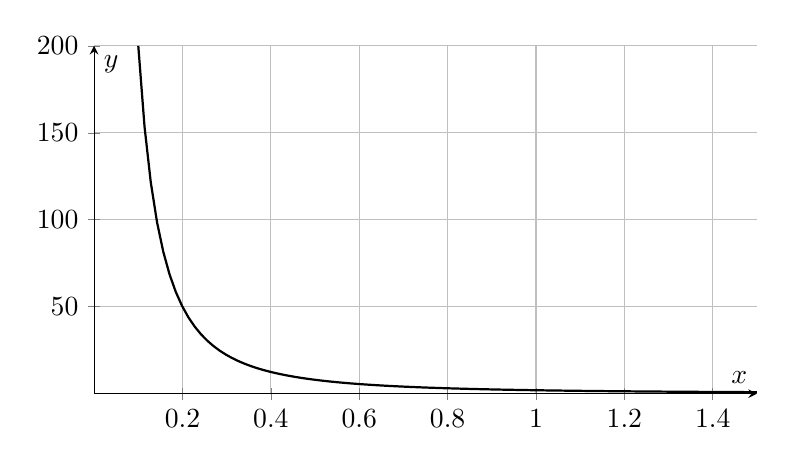
\begin{tikzpicture}
\begin{axis}[
    axis lines = middle,
    xlabel = $x$,
    ylabel = $y$,
    grid = both,
    width=10cm,
    height=6cm,
    xmin=0, xmax=1.5,
    ymin=0, ymax=200
]
\addplot [domain=0.1:1.5, samples=100, black, thick] {2/(x^2)};
\end{axis}
\end{tikzpicture}
\end{center}

When \(l^2 < 2mA\)
\begin{center}
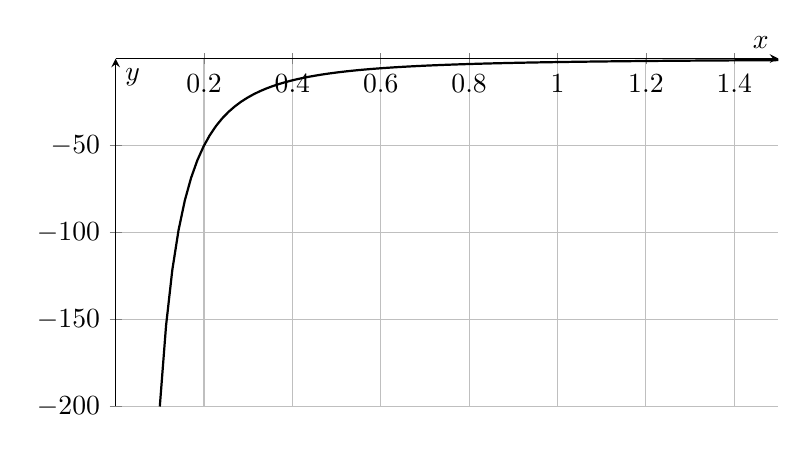
\begin{tikzpicture}
\begin{axis}[
    axis lines = middle,
    xlabel = $x$,
    ylabel = $y$,
    grid = both,
    width=10cm,
    height=6cm,
    xmin=0, xmax=1.5,
    ymin=-200, ymax=0
]
\addplot [domain=0.1:1.5, samples=100, black, thick] {-2/(x^2)};
\end{axis}
\end{tikzpicture}
\end{center}

When \(l^2 = 2mA\), \(U_{\text{eff}}(r) = 0 \ \forall \ r\)

\subsubsection*{(b)}
Uniform radial velocity i.e. \(\ddot{r} = 0\)
\[
ma_r = F(r)
\]
\[
m(\ddot{r} - r\dot{\theta}^2) = - \frac{2A}{r^3}
\]
\begin{align*}
    \ddot{r} &= r\dot{\theta}^2 - \frac{2A}{mr^3} \\
    &= r\left(\frac{l^2}{m^2r^4}\right) - \frac{2A}{mr^3} \\
    &= 0
\end{align*}
\[
\Rightarrow l^2 = 2mA
\]
\[
\Rightarrow l = \sqrt{2mA}
\]

\subsubsection*{(c)}
\[
\dot{\theta} = \frac{l}{mr^2} = \frac{\sqrt{2mA}}{mr^2}
\]
\[
\dot{\theta} = \frac{d\theta}{dr} \frac{dr}{dt}
\]
\[
\Rightarrow \frac{d\theta}{dr} = \frac{\sqrt{2mA}}{mvr^2}
\]
\[
\Rightarrow \theta = \frac{\sqrt{2mA}}{mv} \int \frac{1}{r^2} dr
\]
\[
\Rightarrow \theta = -\frac{\sqrt{2mA}}{mvr} + \theta_0
\]










\subsection*{Question 3}
\[
\ddot{I} + 6 \dot{I} + 8I = Ce^{-t}
\]
\subsubsection*{(a)}
Guess \(I(t) = e^{\lambda t}\)
\[
\Rightarrow (\lambda^2 + 6\lambda + 8)e^{\lambda t} = 0
\]
Since \(e^{\lambda} \neq 0, \ \forall \ t\)
\[
\Rightarrow \lambda^2 + 6 \lambda + 8 = 0
\]
Thus \(\lambda = -4\) or \(\lambda = -2\)

\[
\Rightarrow I(t) = Ae^{-4t} + Be^{-2 t}
\]

\subsubsection*{(b)}
Guess particular solution \(I(t) = \alpha e^{-t}\)
\[
\Rightarrow \alpha e^{-t} - 6\alpha e^{-t} + 8\alpha e^{-t} = 6e^{-t}
\]
\[
\Rightarrow \alpha = 2
\]
Thus the particular solution is \(I(t) = 2e^{-t}\)

\subsubsection*{(c)}
To find the general solution, we simply add the general solution and the particular solution together
\[
\Rightarrow I(t) = Ae^{-4t} + Be^{-2 t} + 2e^{-t}
\]

\subsection*{Question 4}

First I will compute the moment of inertia of a ring with outer radius \(r_2\) and
inner radius \(r_1\)
\[
I_0 = \int_{\text{object}} r^2 dm
\]
\[
dm = \lambda r dr d \theta, \quad \lambda = \frac{M}{\pi (r_2^2 - r_1^2)}
\]
\begin{align*}
    I_0 &= \frac{M}{\pi (r_2^2 - r_1^2)}\int_{0}^{2\pi} \int_{r_1}^{r_2} r^3 dr d\theta \\
    &= \frac{M}{2(r_2^2 - r_1^2)}(r_2^4 - r_1^4) \\
    &= \frac{M}{2}(r_2^2 + r_1^2)
\end{align*}

\subsubsection*{(a)}
For a circle \(r_2 = r_1 = R\)
\[
\Rightarrow I_0 = MR
\]

\subsubsection*{(b)}
For a solid disk \(r_1 = 0\), \(r_2 = R\)
\[
\Rightarrow I_0 = \frac{MR}{2}
\]
\end{document}